\documentclass[11pt]{article}
\usepackage{amsfonts, amssymb, amsmath, graphicx}
\usepackage{multirow}
\usepackage{tikz}
\usepackage{subcaption} 

\usetikzlibrary{positioning, shapes.multipart} 
\oddsidemargin=-0.5cm
\setlength{\textwidth}{6.5in}
\addtolength{\voffset}{-20pt}
\addtolength{\headsep}{25pt}

\pagestyle{myheadings}
\markright{Xin Zhou \hfill CS184 Homework1 \hfill}

\begin{document}
%%%%%%%%%%%%%%%%%%%%%%%%%%%%%%%%%%%%%%%%%%%%%%%%%%%%%%%%%%%%%%%%%%%%%%%%%%%%%%%%
\subsection*{Task 1 Drawing Single-Color Triangles}
\begin{figure}[h]
    \centering
    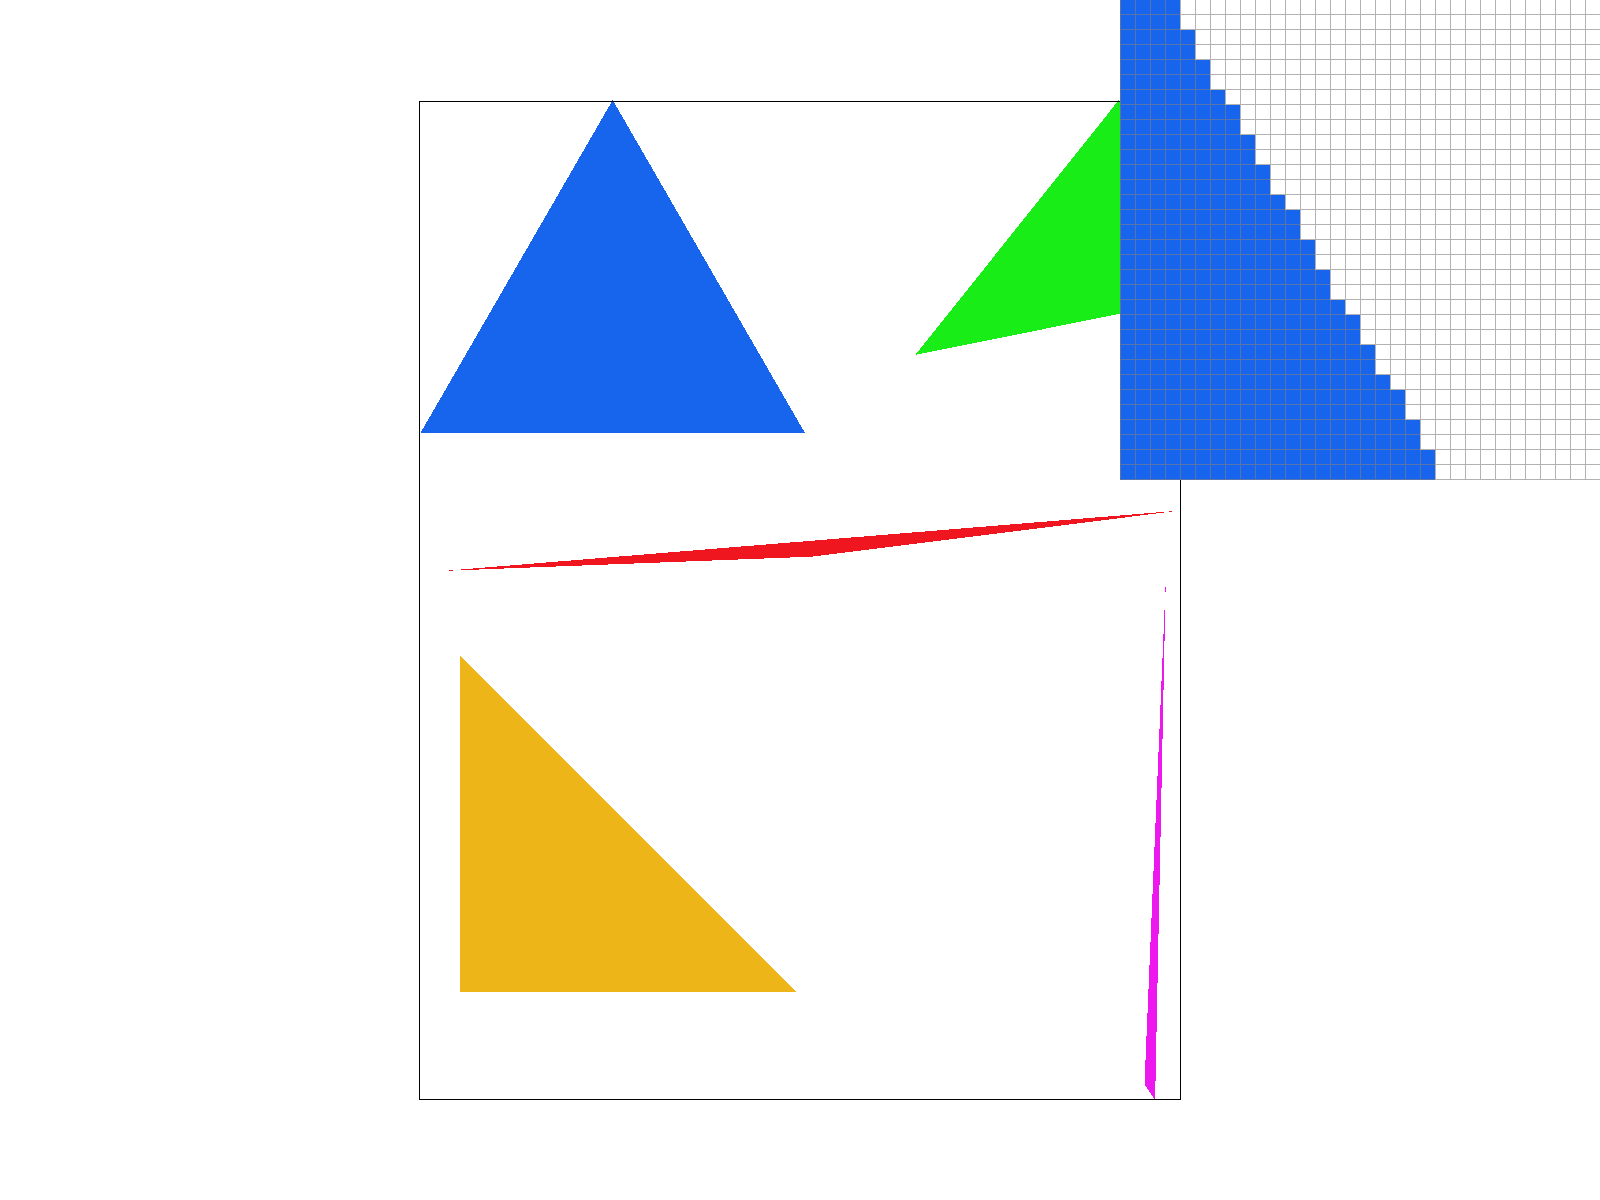
\includegraphics[width=0.9\textwidth]{T1.png} 
    \caption{\text{The output of Task 1 with highlighed area of aliasing}}% Replace with your file name
\end{figure}
In order to draw a continuous colored triangle to the screen space
with discrete pixels, we need to sample if each pixel center is inside this
triangle. In \texttt{rasterize\_triangle()}, the basic idea is
to use nested \texttt{for} loop to walk through each pixel, then if
the center of a pixel is \texttt{inside\_triangle(x+0.5, y+0.5)}, \texttt{fill\_pixel()} will be called.
\begin{verbatim}
  //pseudocode
  for (x {0}; x < width; ++x)
    for (y {0}; y < height; ++y) {
      if (inside_triangle(tri, x+0.5, y+0.5)) {
        fill_pixel();}}
\end{verbatim}

The customized \texttt{inside\_triangle()} has a helper function \texttt{line\_test()} to 
calculate $v \cdot N$, which is the dot product of a vector $v$ (from each vertex to the center of a pixel)
and a normal vector $N$ (the normal vector of the oppositing line). Through $v.N >= 0$ on each
line, the center of a pixel is in the triangle for sure.
\begin{figure}[h]
    \centering
    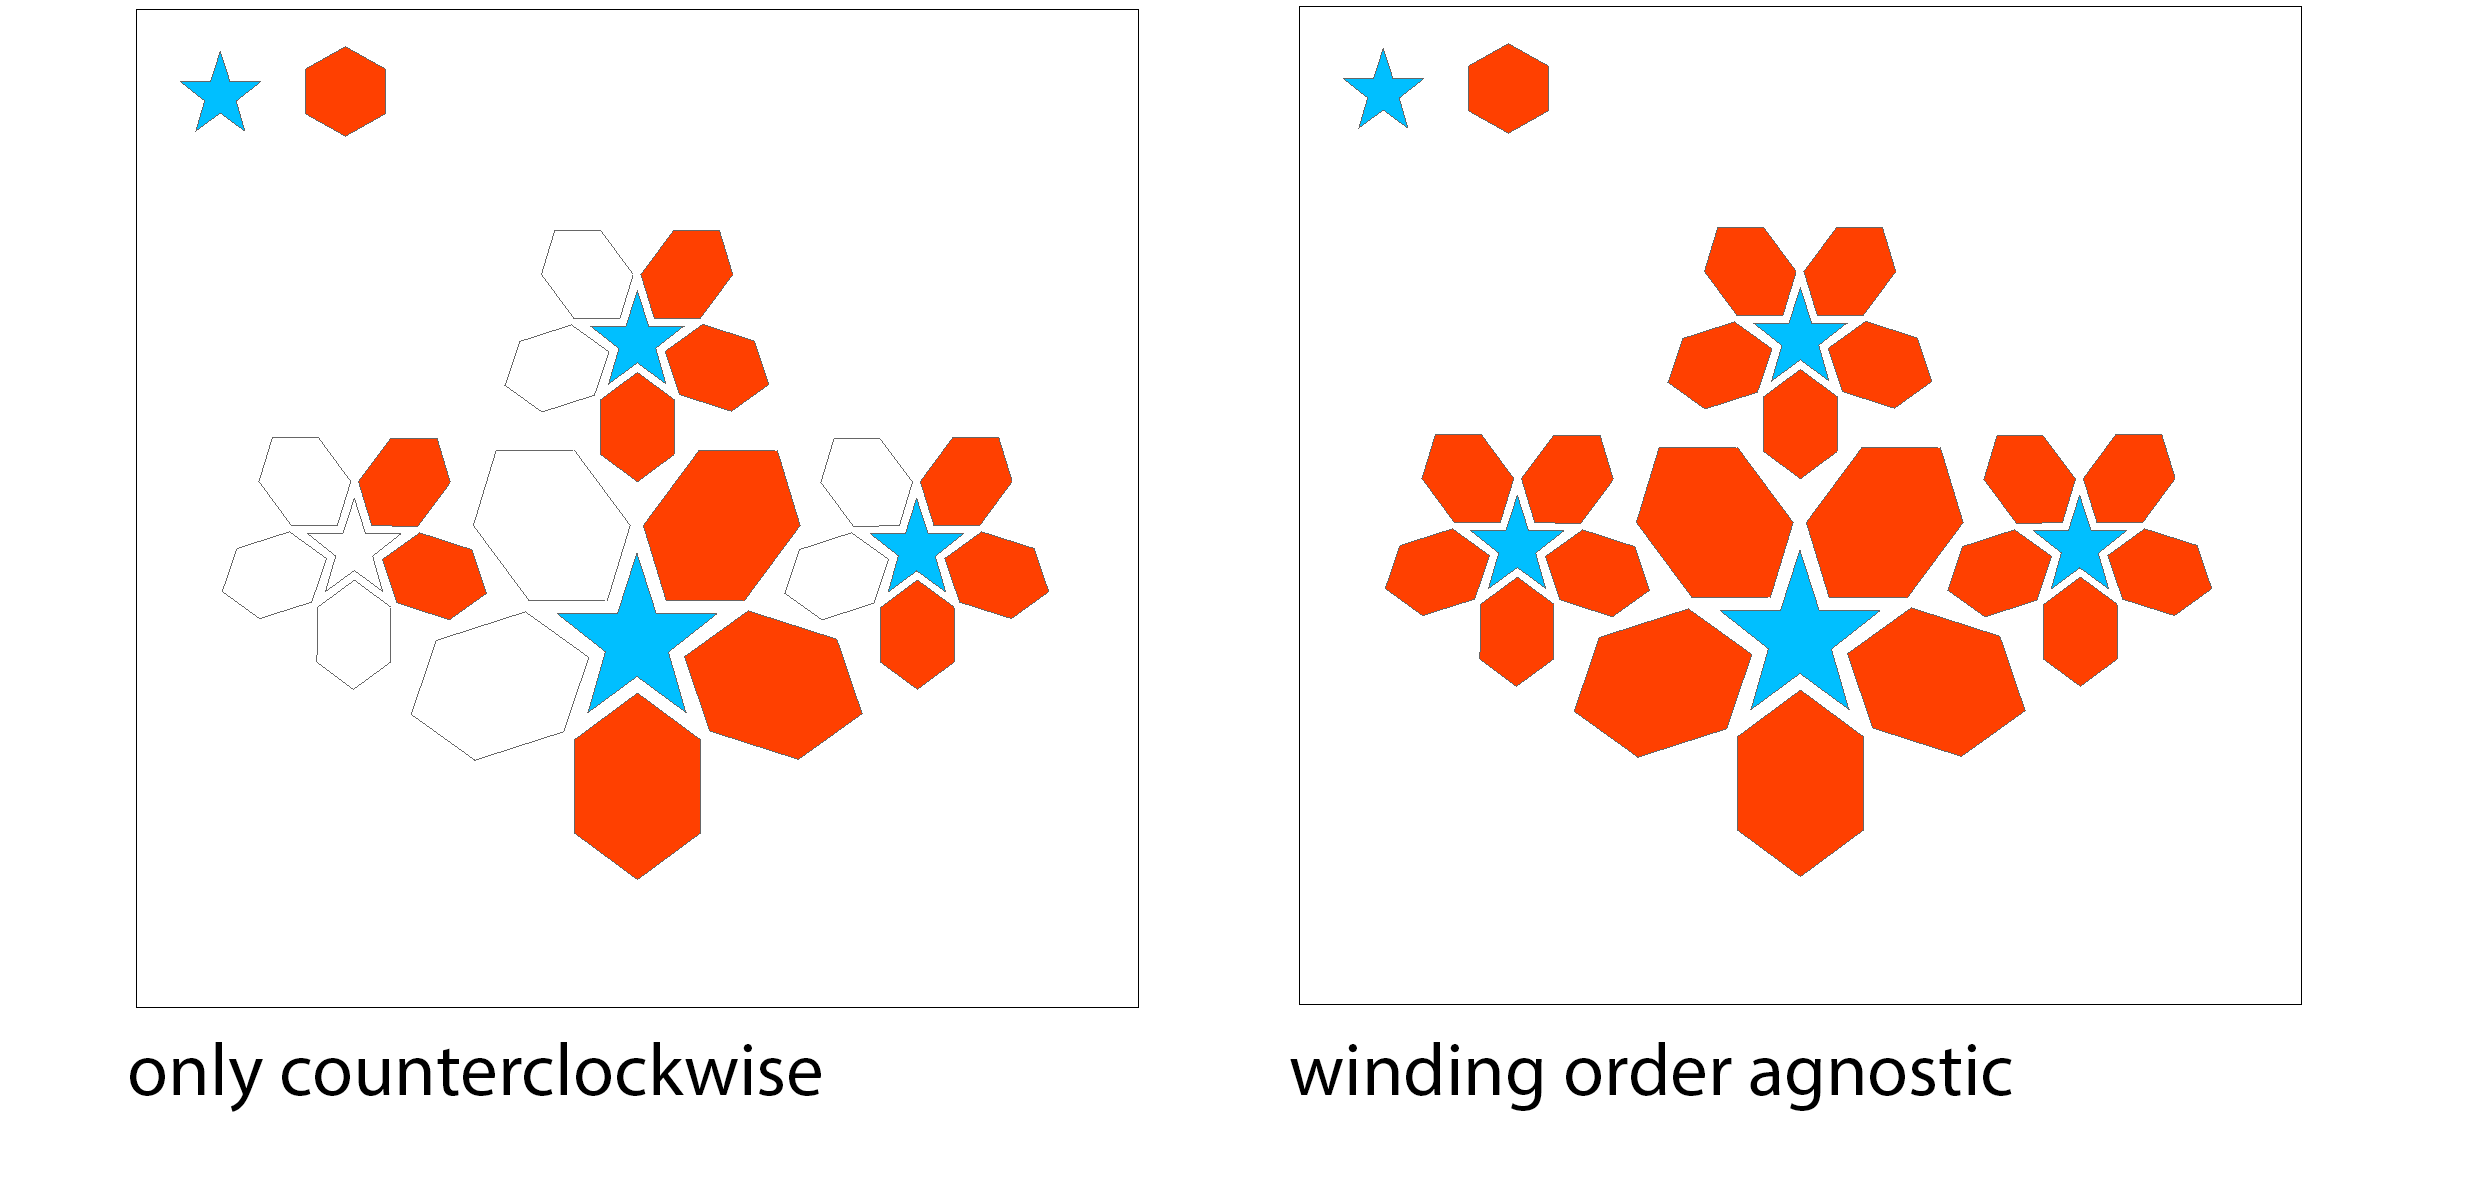
\includegraphics[width=0.8\textwidth]{T13.png} % Replace with your file name
\end{figure}

At the beginning, I only did three line tests using a counterclockwise
order and it ended up in a partially shaded image. By adding another clockwise three line
tests, the function \texttt{inside\_triangle()} became order agnostic.

For efficiency, I use a bounding box approach defined by \texttt{boundingbox()} to limit the
\texttt{for} loop within a rectangle that contains the entire triangle.
This way can avoid checking each pixel in an image that is not intended to be rendered.
To find the \texttt{width} and \texttt{height} of the bounding box, I firstly
found \texttt{min/max x} and \texttt{min/max y} of the three vertices.

\begin{verbatim}
    float max_x = std::max({x0, x1, x2});
    float min_x = std::min({x0, x1, x2});
    float max_y = std::max({y0, y1, y2});
    float min_y = std::min({y0, y1, y2});
\end{verbatim}

However, these values are \texttt{float} and thus cannot be used in calculating loop bounds.
Accordingly, I use \texttt{floor(min x/y)} and \texttt{ceil(max x/y)} and \texttt{clamp}
them to the current \texttt{width} and \texttt{height} of the image to get rid of
out-of-bound issues.

\begin{verbatim}
    int x_start = std::max(0, (int)std::floor(min_x));
    int x_end   = std::min((int)width - 1, (int)std::ceil(max_x));
    int y_start = std::max(0, (int)std::floor(min_y));
    int y_end   = std::min((int)height - 1, (int)std::ceil(max_y));
\end{verbatim}

Then, in the main function \texttt{rasterize\_triangle()}, calling 
\texttt{boundingbox()} will return \texttt{x\_start, x\_end, y\_start, y\_end} and
we can replace the for loop with the new shortened bounds:
\begin{verbatim}
  //pseudocode
  for (int x = x_start; x <= x_end; ++x)
      for (int y = y_start; y <= y_end; ++y) {
        if (inside_triangle(tri, x+0.5, y+0.5)) {
          fill_pixel();}}
\end{verbatim}

Using this method will speed up computation by exluding a lot of unrendered pixels and
avoiding uncecessary arthimetic operations in \texttt{inside\_triangle()}.

For extra credit, I implemented a Tiled Triangle Traversal optimization
mentioned in the class. The bouding box method can still include a lot of leftover
pixels that are outside the triangle. Instead of checking every pixel individually, I divide the bounding box into 4x4 pixel blocks.
For each block, I check if all pixels are inside the triangle (“all in”) or all are outside (“all out”)
by using a variable \texttt{int inside\_sum}.
\begin{verbatim}
  int blocksize = 4;
  for (int x = x_start; x <= x_end; x+=blocksize)
    for (int y = y_start; y <= y_end; y+=blocksize)
    {
      int inside_sum = 0;
      for (int i {0}; i < blocksize; ++i)
        for (int j {0}; j < blocksize; ++j) {
          int block_x = x + i;
          int block_y = y + j;
          // bound check
          if (block_x > b_box[1] || block_y > b_box[3]) continue;
          if (inside_triangle(block_x + 0.5, block_y + 0.5, x0, y0, x1, y1, x2, y2))
          {
            inside_sum++;
          }
      }
      //partial coverage
      if (inside_sum != 0 && inside_sum < blocksize * blocksize)
      {
        for loop in block: 
          if inside_triangle()
              fill_pixel()
      }
      //full coverage
      else if (inside_sum == blocksize * blocksize)
        {
          for loop in block:
            fill_pixel(); 
        }}}
\end{verbatim}
If all are inside, I fill all pixels in the block without \texttt{inside\_triangle()} checks.
If all are outside, I skip the block entirely.
If partially covered, I fall back to the normal sampling method as mentioned before.
This approach skips large empty regions and quickly fills large covered regions, improving performance for large triangles.
\begin{figure}[h]
    \centering
    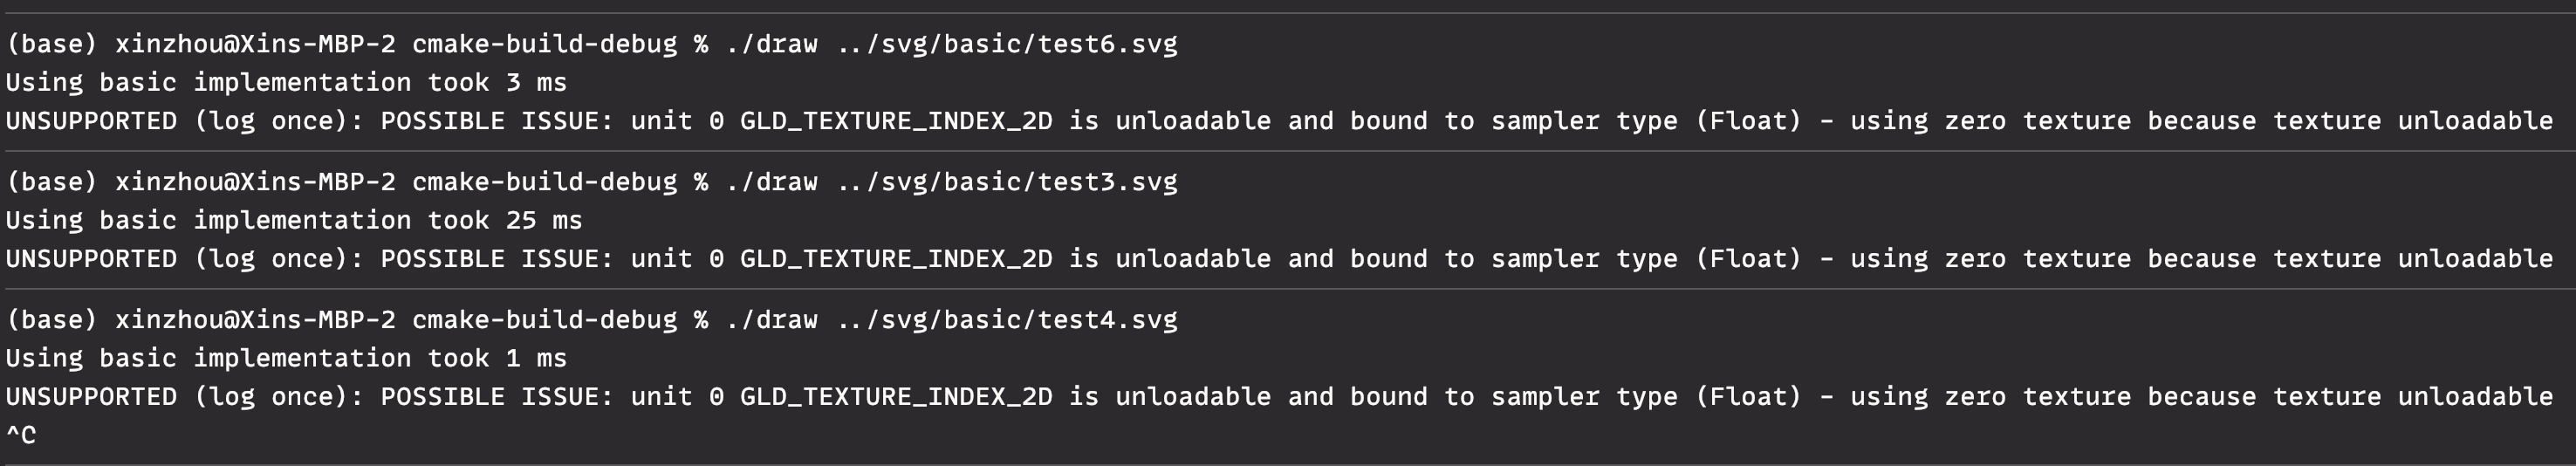
\includegraphics[width=0.99\textwidth]{T14.png}
    \caption{\text{The performance of Bounding box method}}
    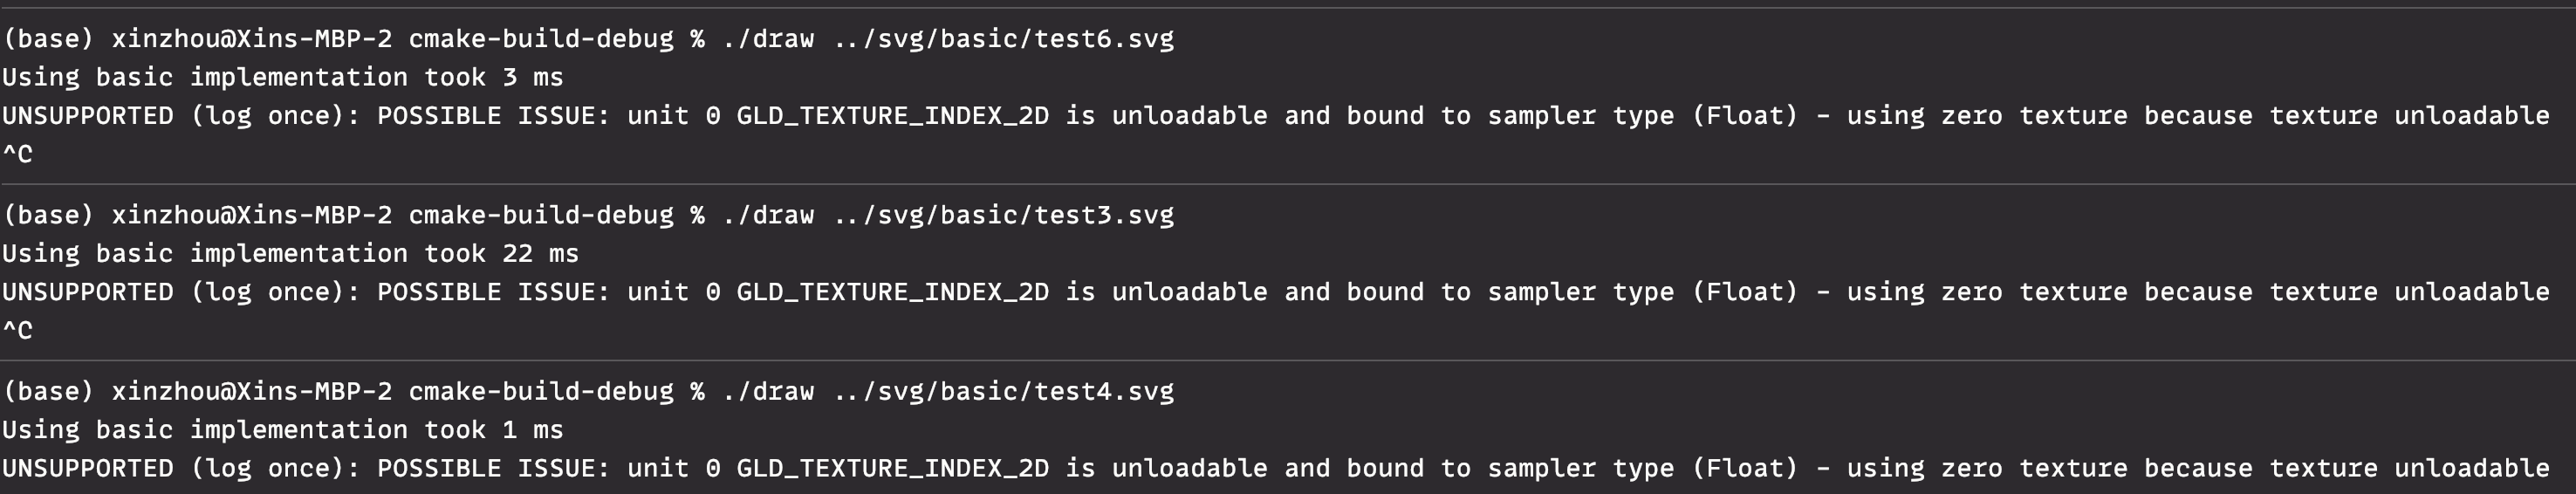
\includegraphics[width=0.99\textwidth]{T15.png}
    \caption{\text{The performance of Bounding box method with Tiled Triangle Traversal}} % Replace with your file name
\end{figure}

From the screenshots, we can see that the optimization can slightly speed up the rendering
for \texttt{test3.svg} from 25ms to 22ms. (Sorry, I used supersampling for this performance test since
I did this extra credit later). I assume the size of triangles matter here because
8*8 block size unexpectedly slowed down the performance since it always fall back to the normal sampling
method with more for loops.
\newpage
%%%%%%%%%%%%%%%%%%%%%%%%%%%%%%%%%%%%%%%%%%%%%%%%%%%%%%%%%%%%%%%%%%%%%%%%%%%%%%%%
\subsection*{Task 2: Antialiasing by Supersampling}
Similar to Task 1, I still loop through the bounding box and call a helper function
\texttt{Supersample()}.
\begin{verbatim}    
  for (int x {x_start}; x <= x_end; ++x)
      for (int y {y_start}}; y <= y_end; ++y) {
        Supersample(x, y, x0, y0, x1, y1, x2, y2, color);
      }
\end{verbatim}

\begin{figure}[h]
    \centering
    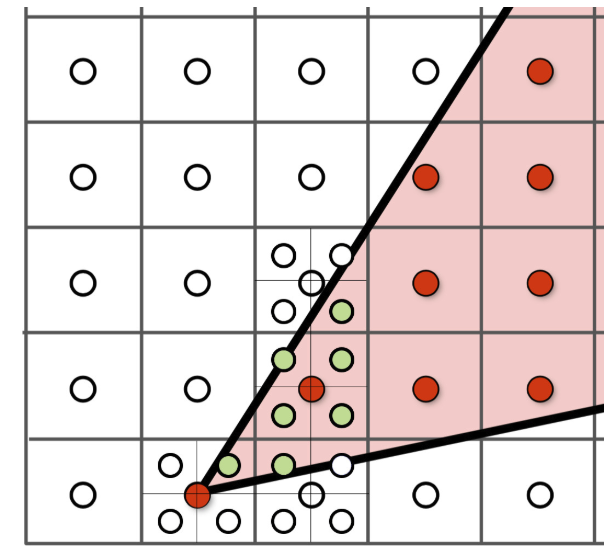
\includegraphics[width=0.40\textwidth]{T2r.png}
    \caption{\text{A supersampling diagram from CS184 hw1}} % Replace with your file name
  \end{figure}

When clicking on "-/+", the \texttt{Supersample()} function will use
the according sample rate to subdivse each screen space pixel into
\texttt{sqrt(sample\_rate) * sqrt(sample\_rate)} subpixels. Then we need to
loop through each subpixel to check if each of them is \texttt{inside\_triangle()}.
However, in the local grid of a pixel, we need to transfer each local center of the subpixel
into the screen space coordinate. In the code below, \texttt{global\_x/y\_center}
are passed into \texttt{inside\_triangle()}.
\begin{verbatim}    
  int local_width = (int)sqrt(sample_rate);

  // loop through the local grid
  for (int i {0}; i < local_width; ++i)
      for (int j {0}; j < local_width; ++j)
      {
        // transfer local position to screen space position
        loat local_x_center = (i + 0.5f) / local_width;
        float local_y_center = (j + 0.5f) / local_width;
        float global_x_center = x + local_x_center;
        float global_y_center = y + local_y_center;

        if (inside_triangle(global_x_center, global_y_center, x0, y0, x1, y1, x2, y2))
        {
          //using row-major 1D array to represent 2D information
          const int index = flatten_2D_index(x, y, i, j, local_width);
          sample_buffer[index] = c;
        }
      }
\end{verbatim}

If the center of a subpixel is inside the triangle, instead of directly calling
\texttt{fill\_pixel()}, \texttt{flatten\_2D\_index()} maps the 2D array into 1D array
and return the index for \texttt{sample\_buffer}, which is a \texttt{vector}.
We can then use \texttt{sample\_buffer[index]} to assign the color efficiently.

In the \texttt{flatten\_2D\_index()} method, we need to use \texttt{y * width + x}
to get the index of the current pixel. 
\begin{verbatim}    
    const int flat_origin = y * width + x;
    const int flat_subpixels = flat_origin * sample_rate + j * local_width + i;
    return flat_subpixels;
\end{verbatim}


\begin{figure}[h]
    \centering
    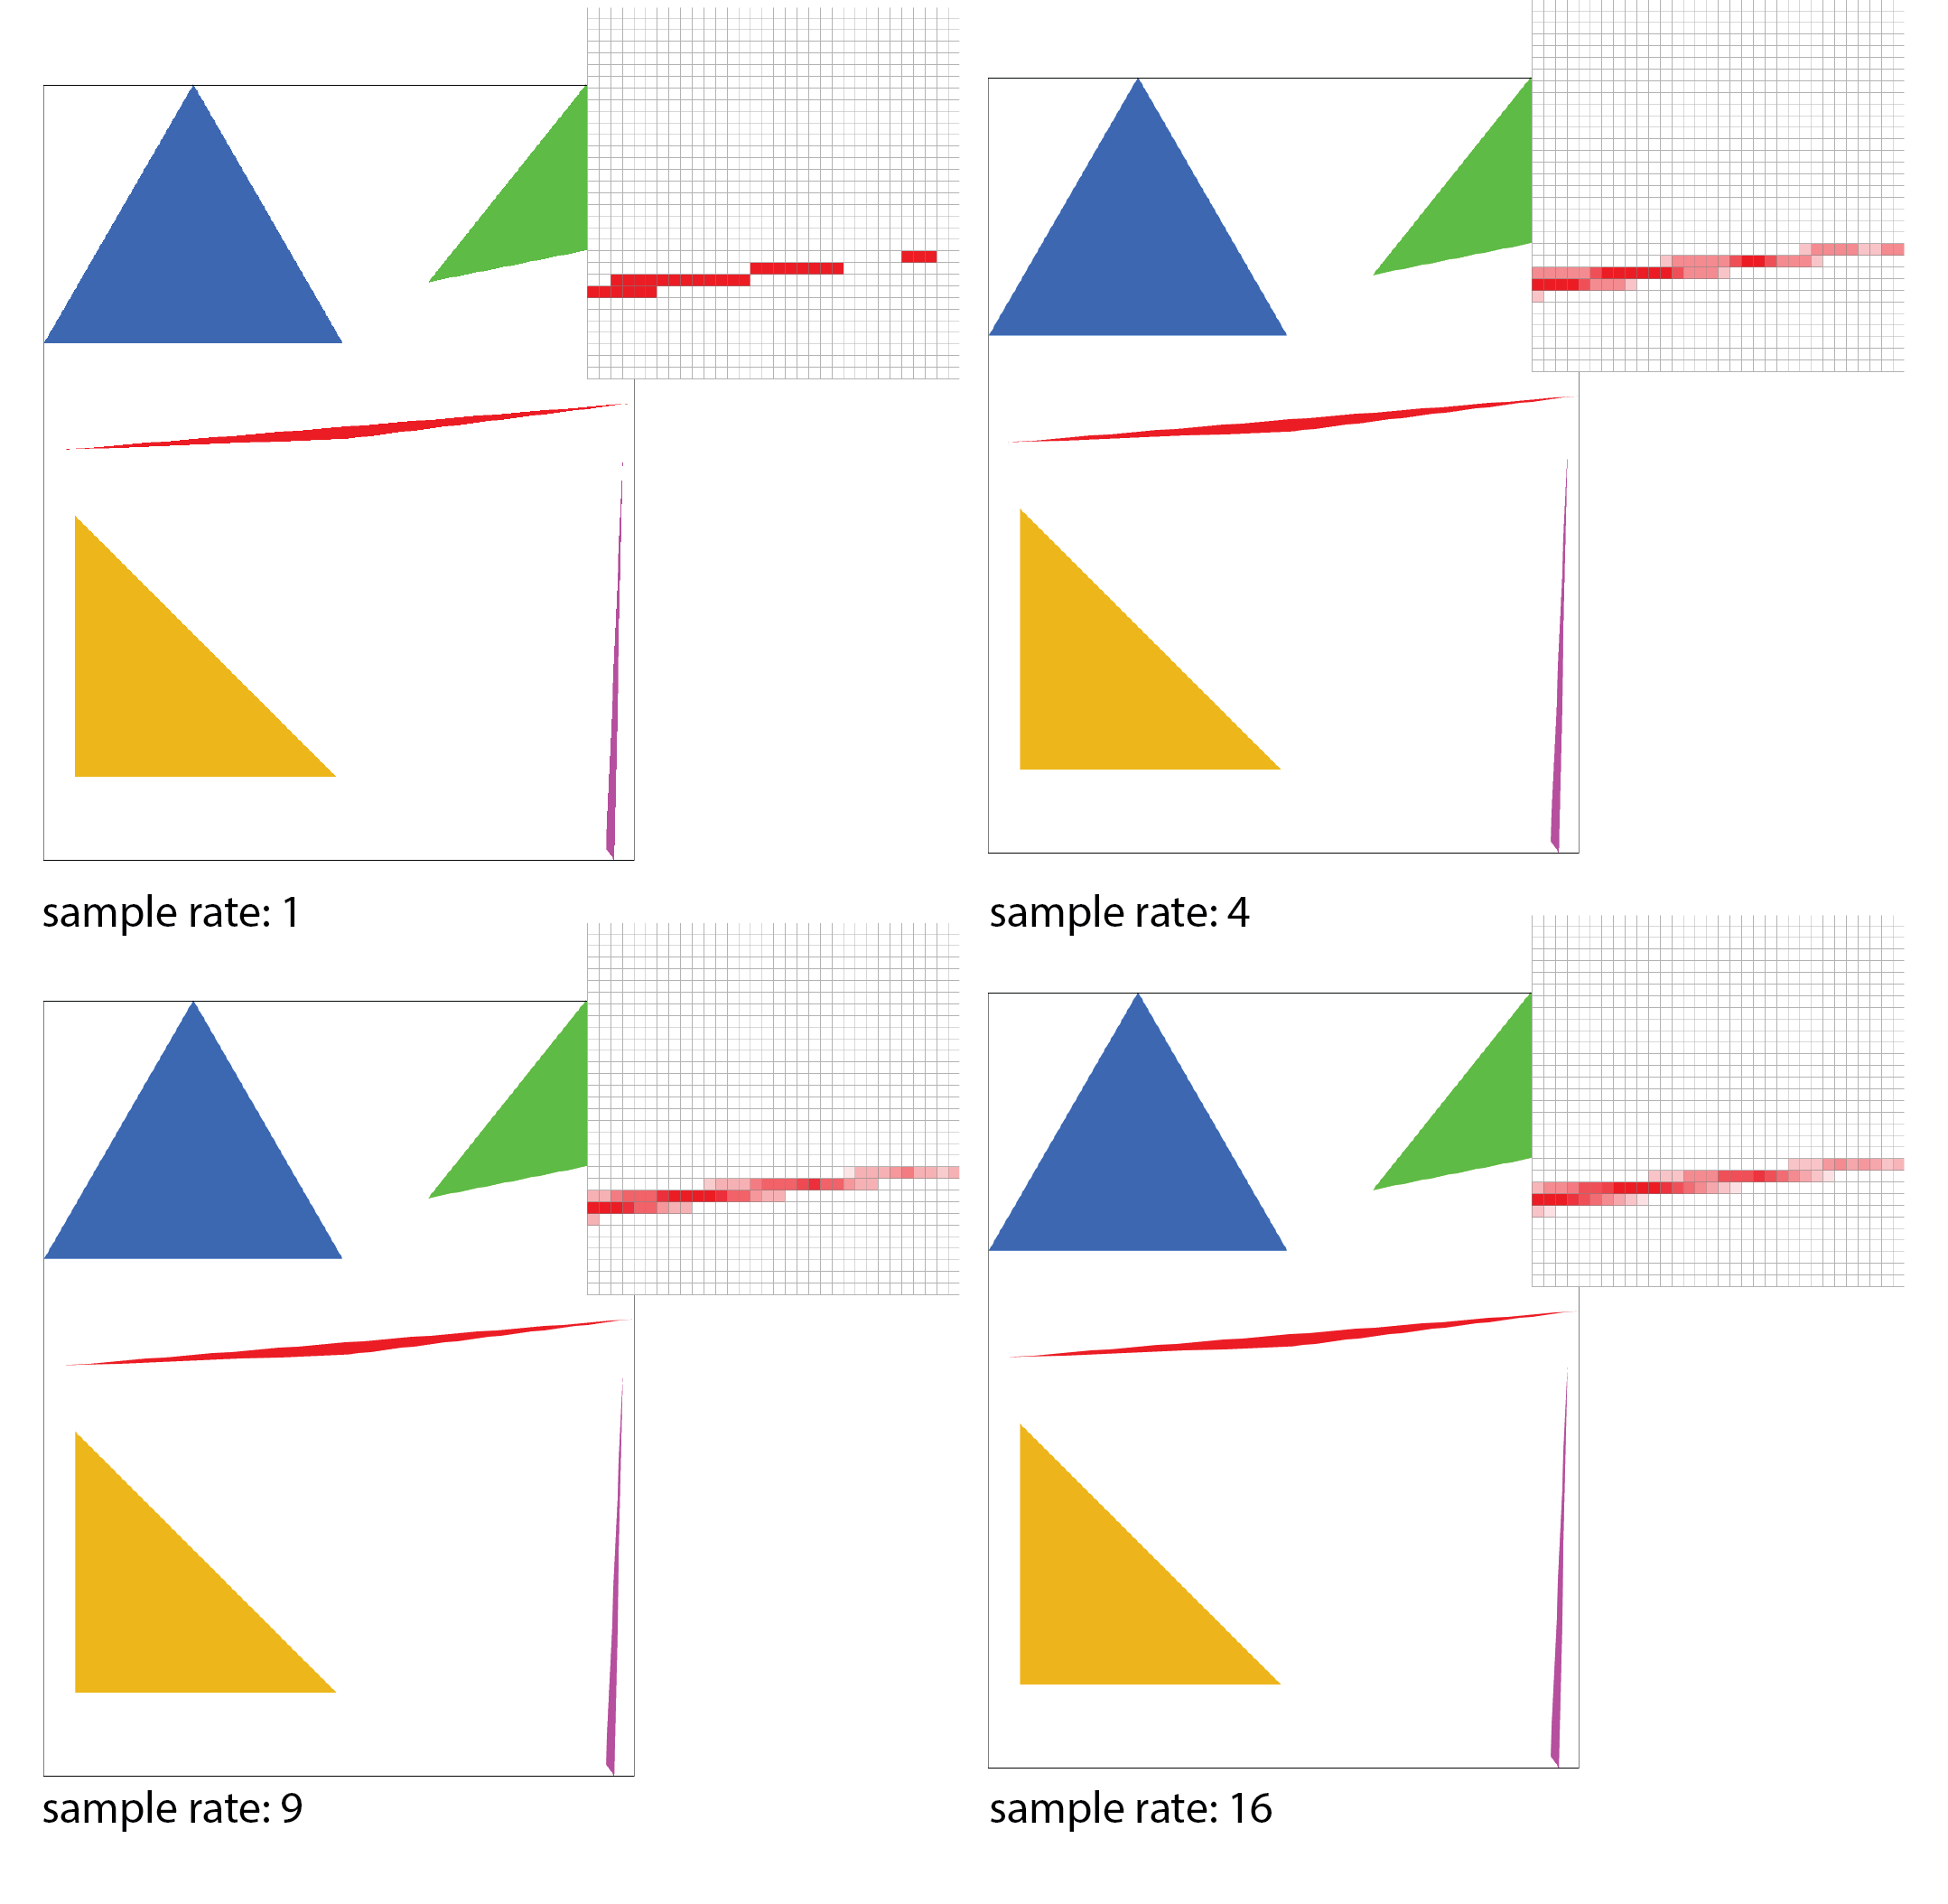
\includegraphics[width=0.90\textwidth]{T2f6.png} % Replace with your file name
  \end{figure}
\newpage
%%%%%%%%%%%%%%%%%%%%%%%%%%%%%%%%%%%%%%%%%%%%%%%%%%%%%%%%%%%%%%%%%%%%%%%%%%%%%%%%
\subsection*{Task 3: Transforms}
\begin{figure}[h]
    \centering
    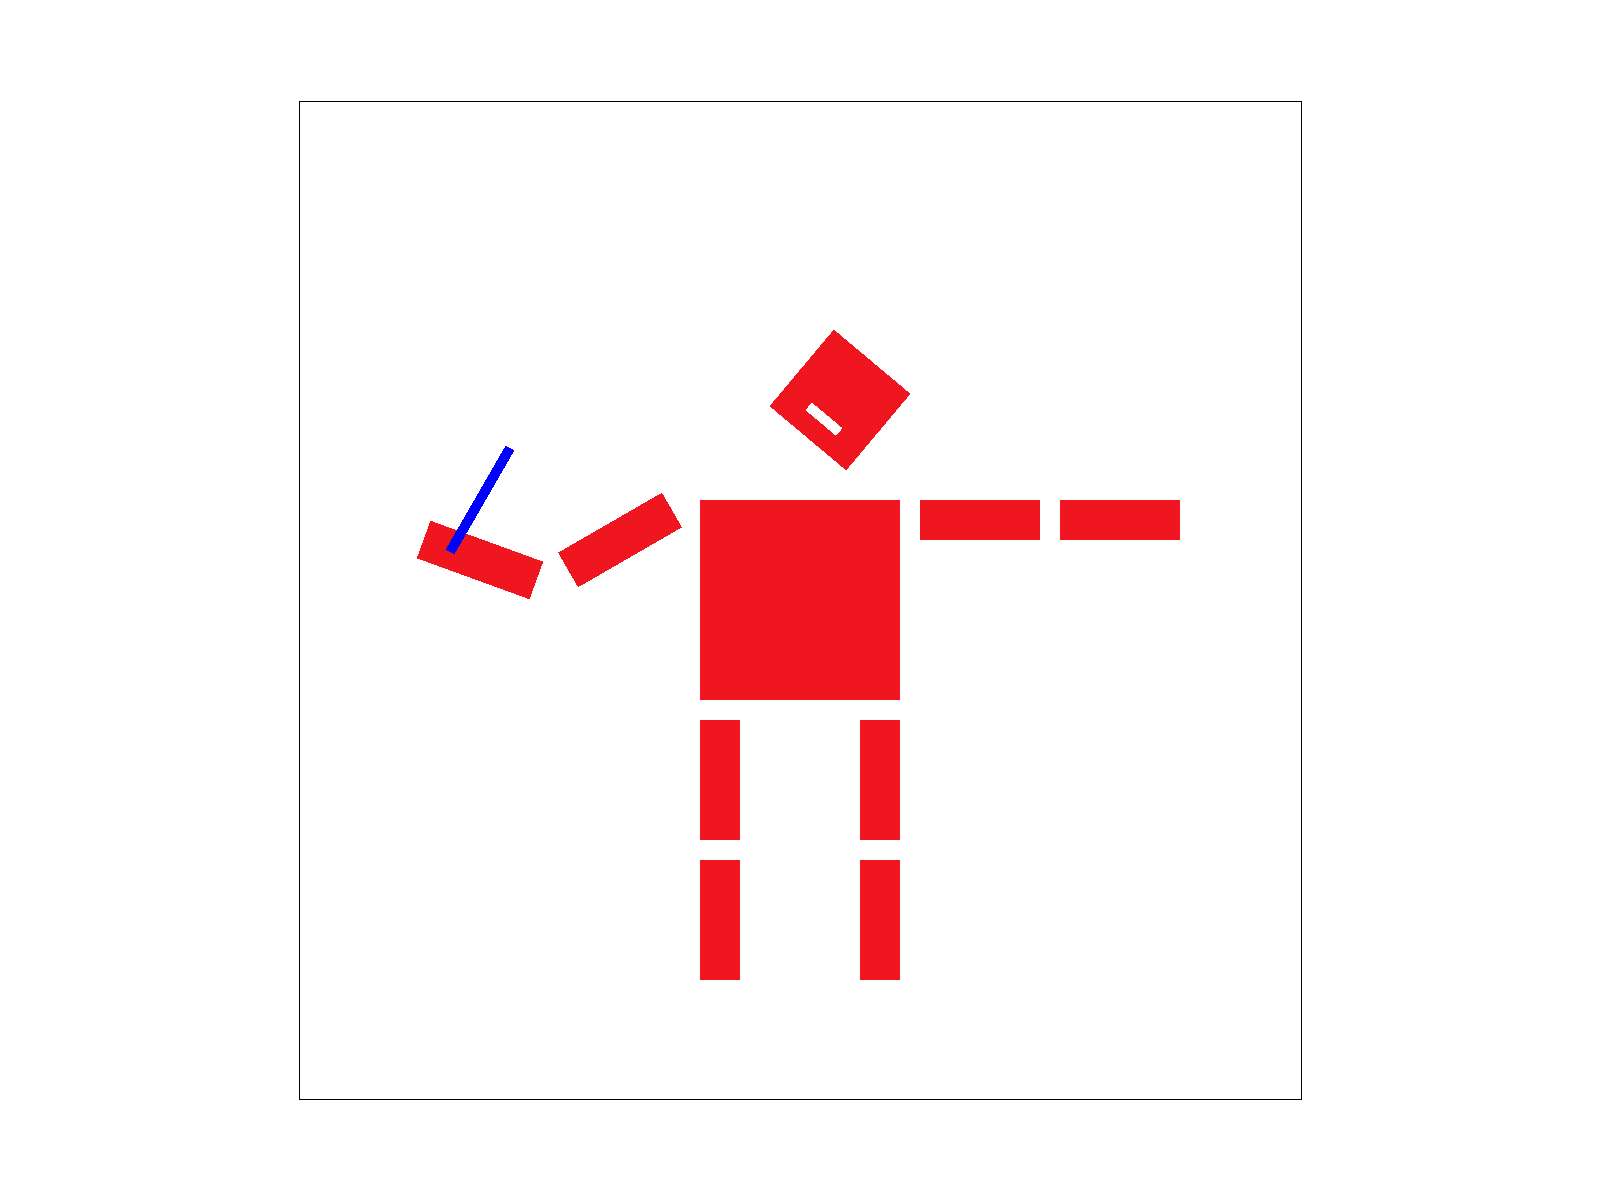
\includegraphics[width=0.95\textwidth]{T3.png} % Replace with your file name
  \end{figure}

  I created a person unhappily looking at a stick in his right hand with his left hand
  pointing to another direction. 

\newpage
%%%%%%%%%%%%%%%%%%%%%%%%%%%%%%%%%%%%%%%%%%%%%%%%%%%%%%%%%%%%%%%%%%%%%%%%%%%%%%%%
\subsection*{Task 4: Barycentric coordinates}
\begin{figure}[h]
    \centering
    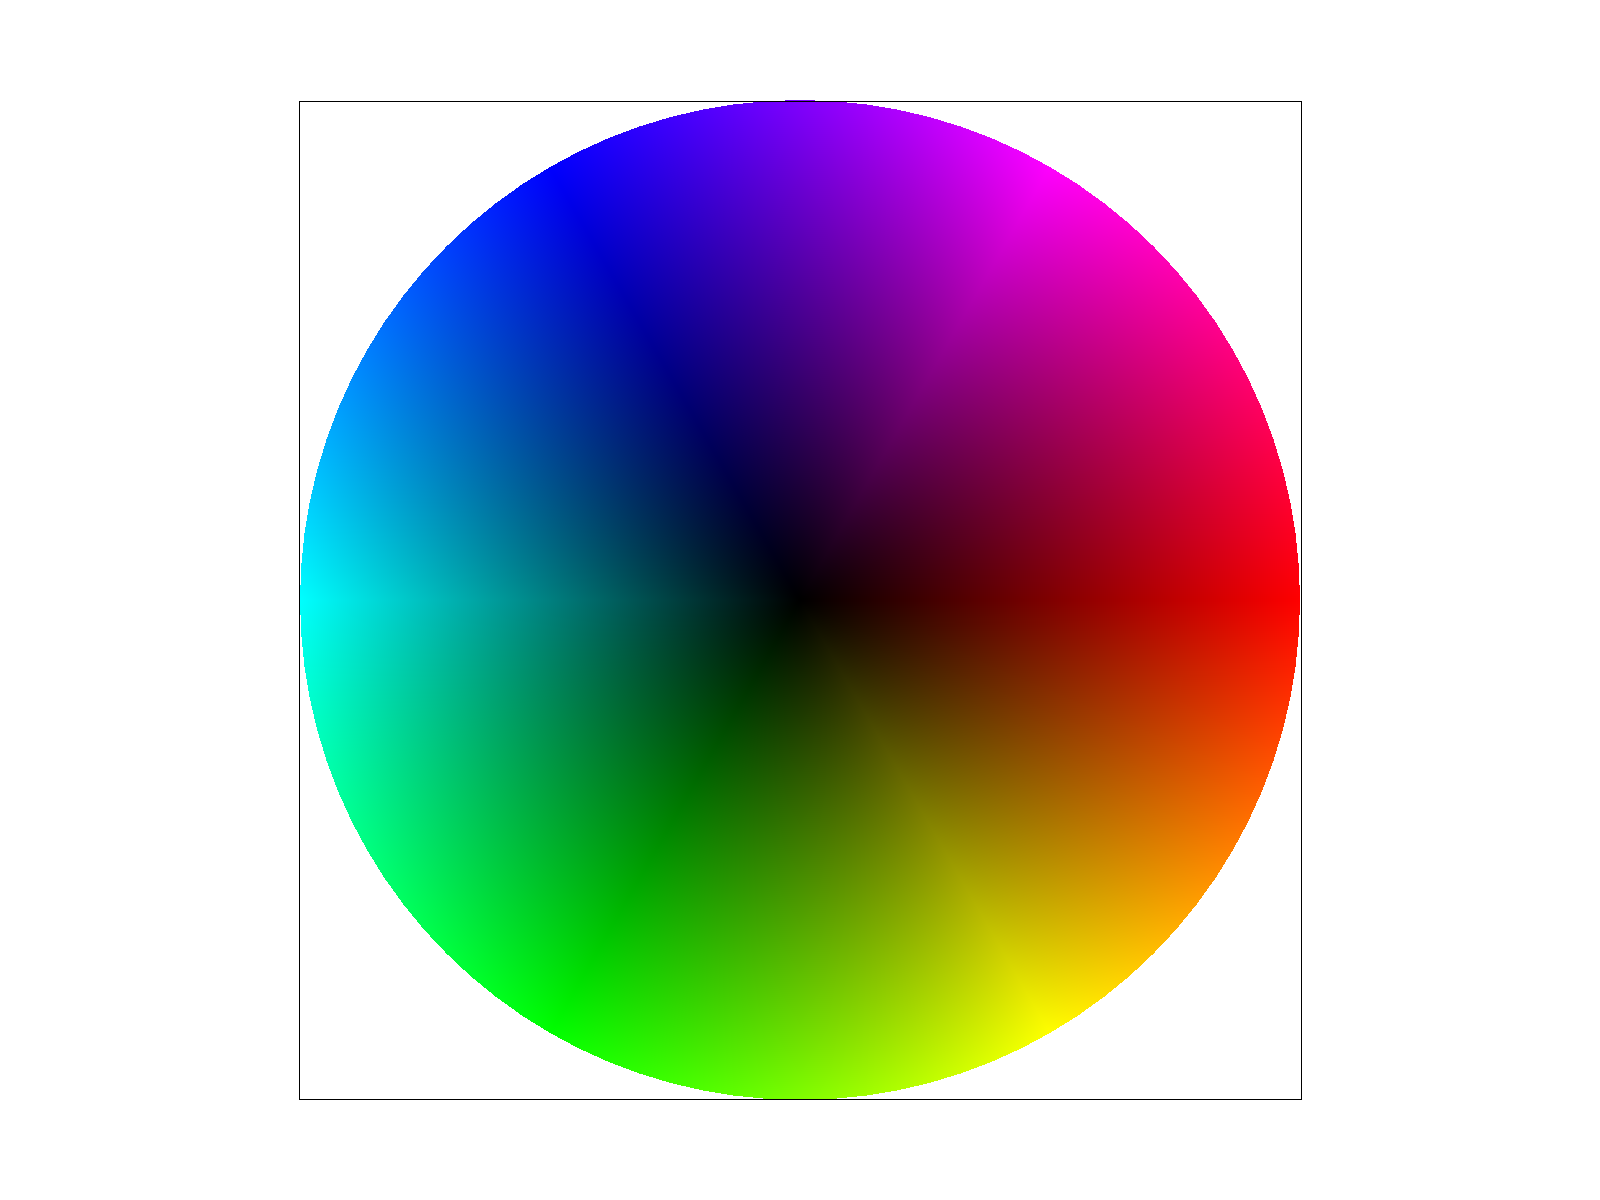
\includegraphics[width=0.95\textwidth]{T4.png} % Replace with your file name
  \end{figure}
\newpage
%%%%%%%%%%%%%%%%%%%%%%%%%%%%%%%%%%%%%%%%%%%%%%%%%%%%%%%%%%%%%%%%%%%%%%%%%%%%%%%%
\subsection*{Task 5: Pixel sampling for texture mapping}
\begin{figure}[h]
    \centering
    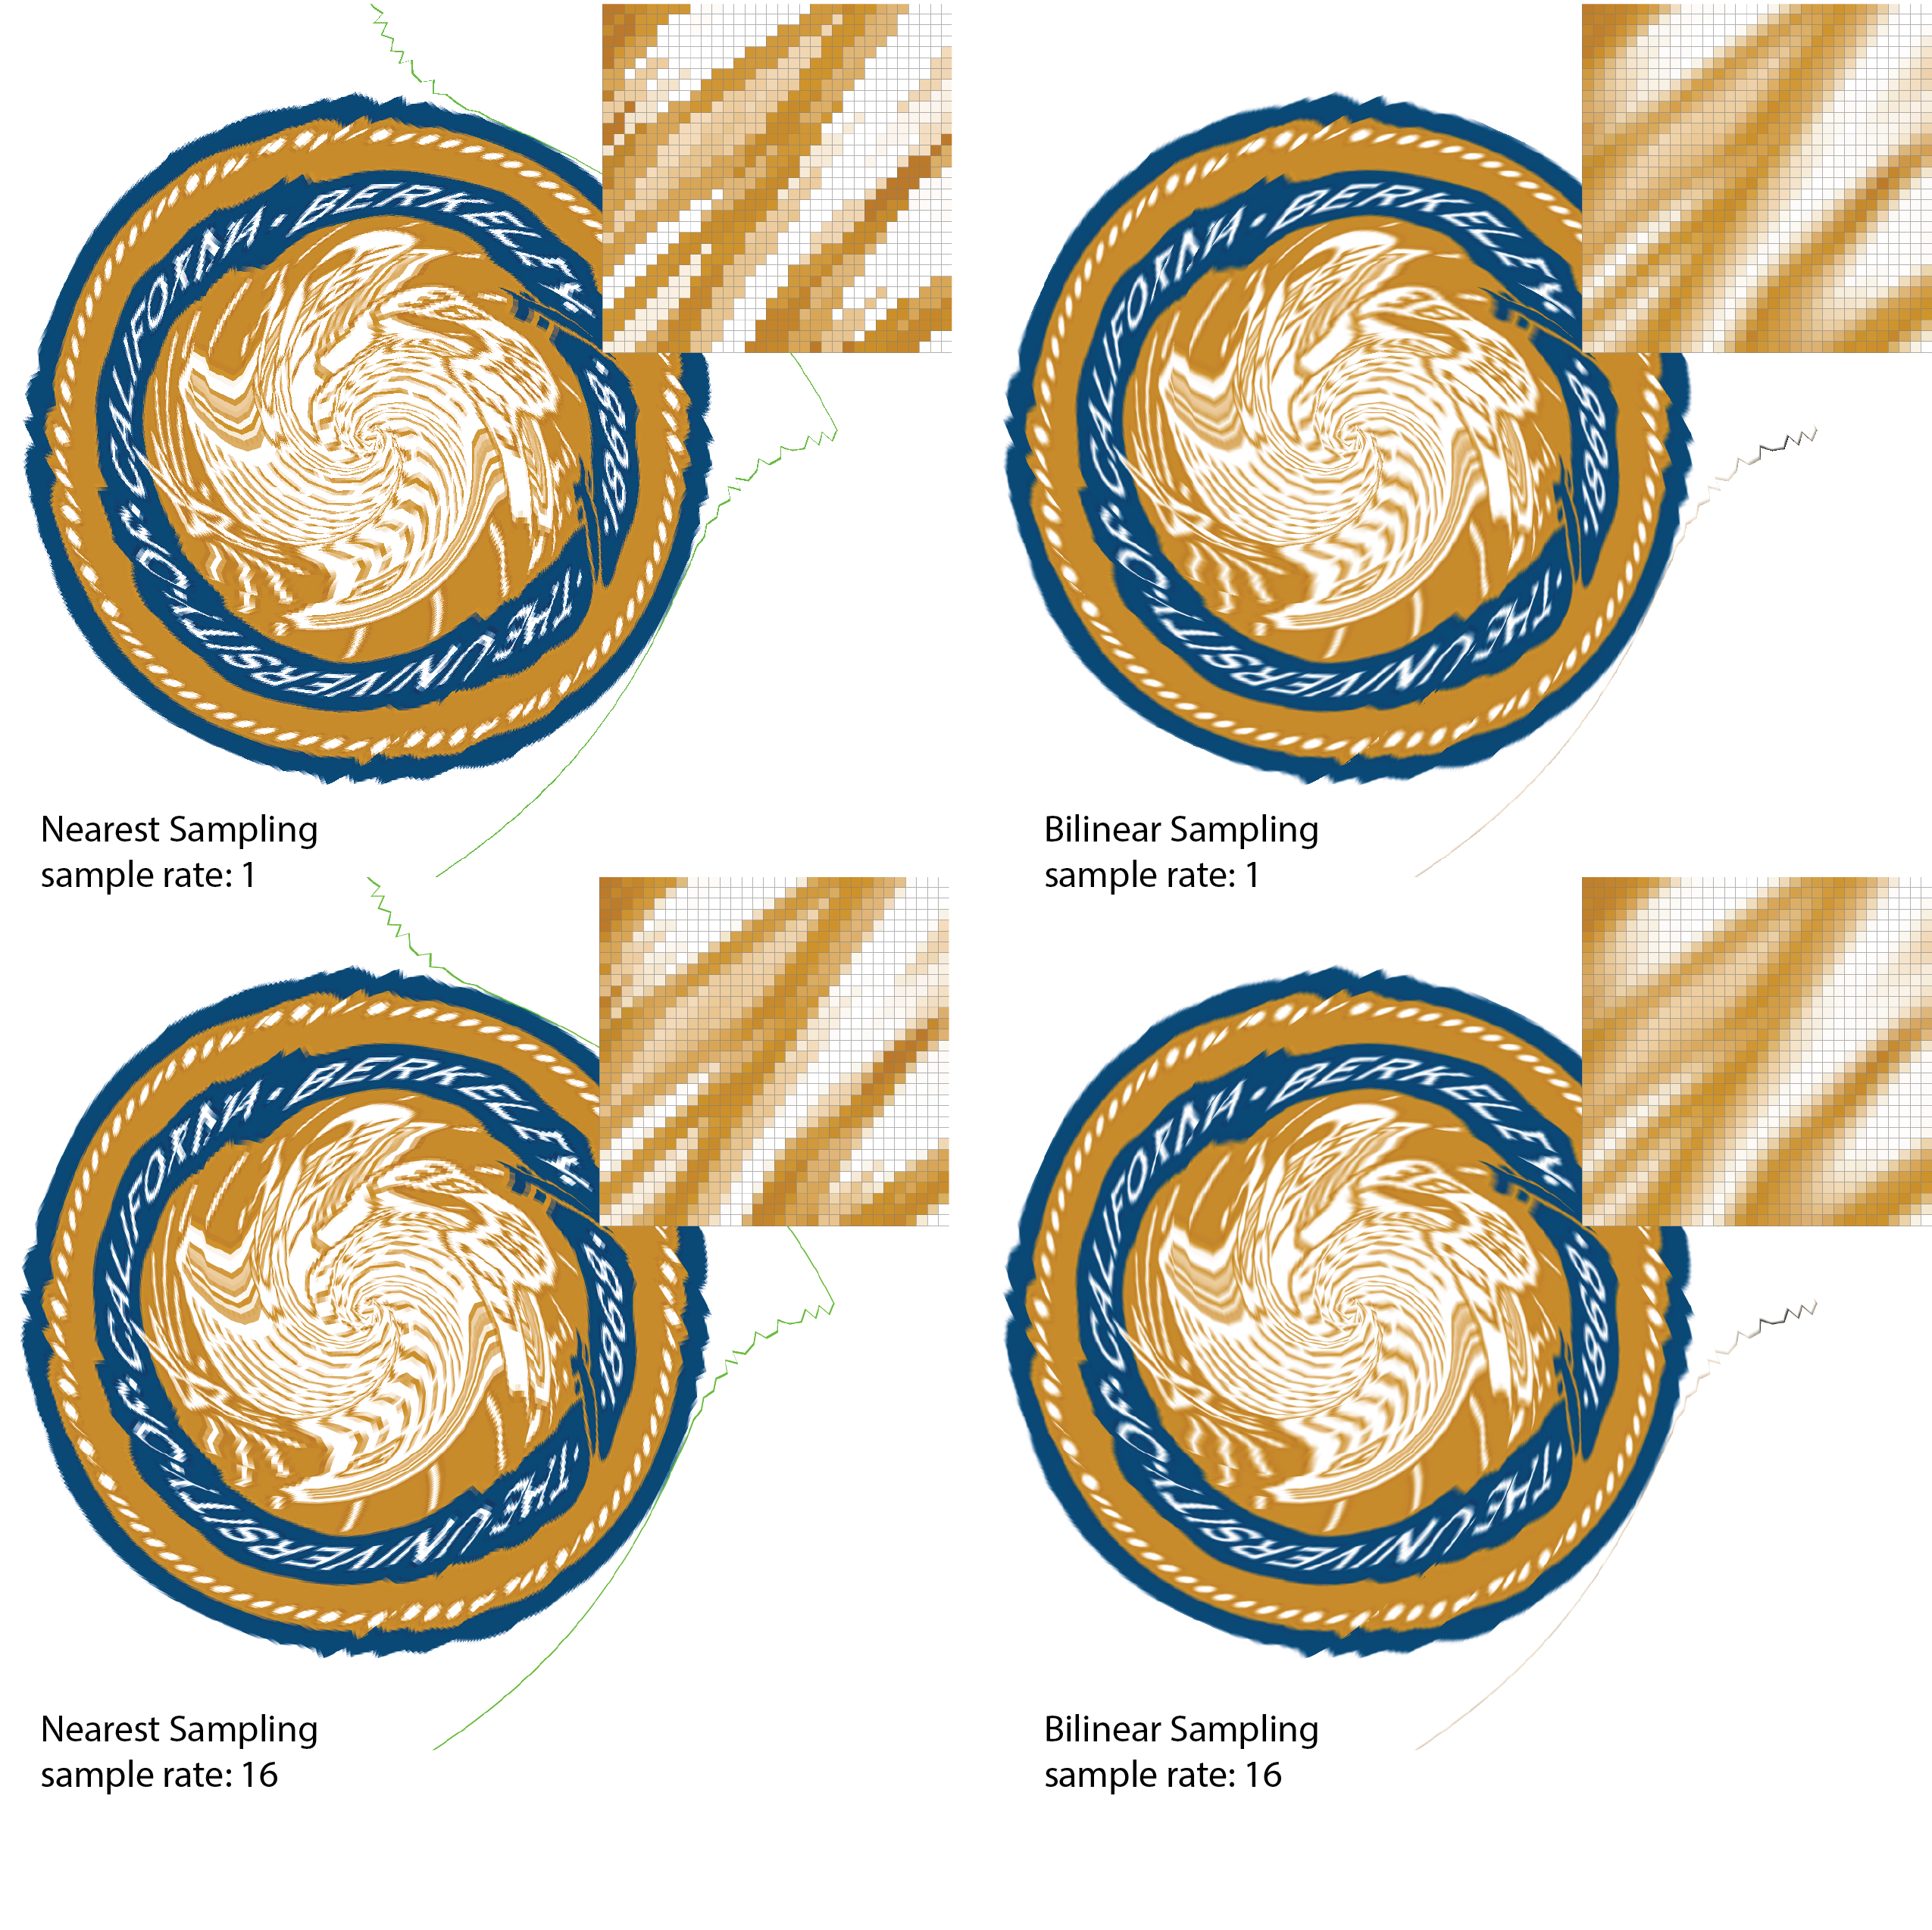
\includegraphics[width=0.89\textwidth]{T5.png} % Replace with your file name
  \end{figure}
\newpage
%%%%%%%%%%%%%%%%%%%%%%%%%%%%%%%%%%%%%%%%%%%%%%%%%%%%%%%%%%%%%%%%%%%%%%%%%%%%%%%%
\subsection*{Task 6: Level sampling with mipmaps for texture mapping}
\begin{figure}[h]
    \centering
    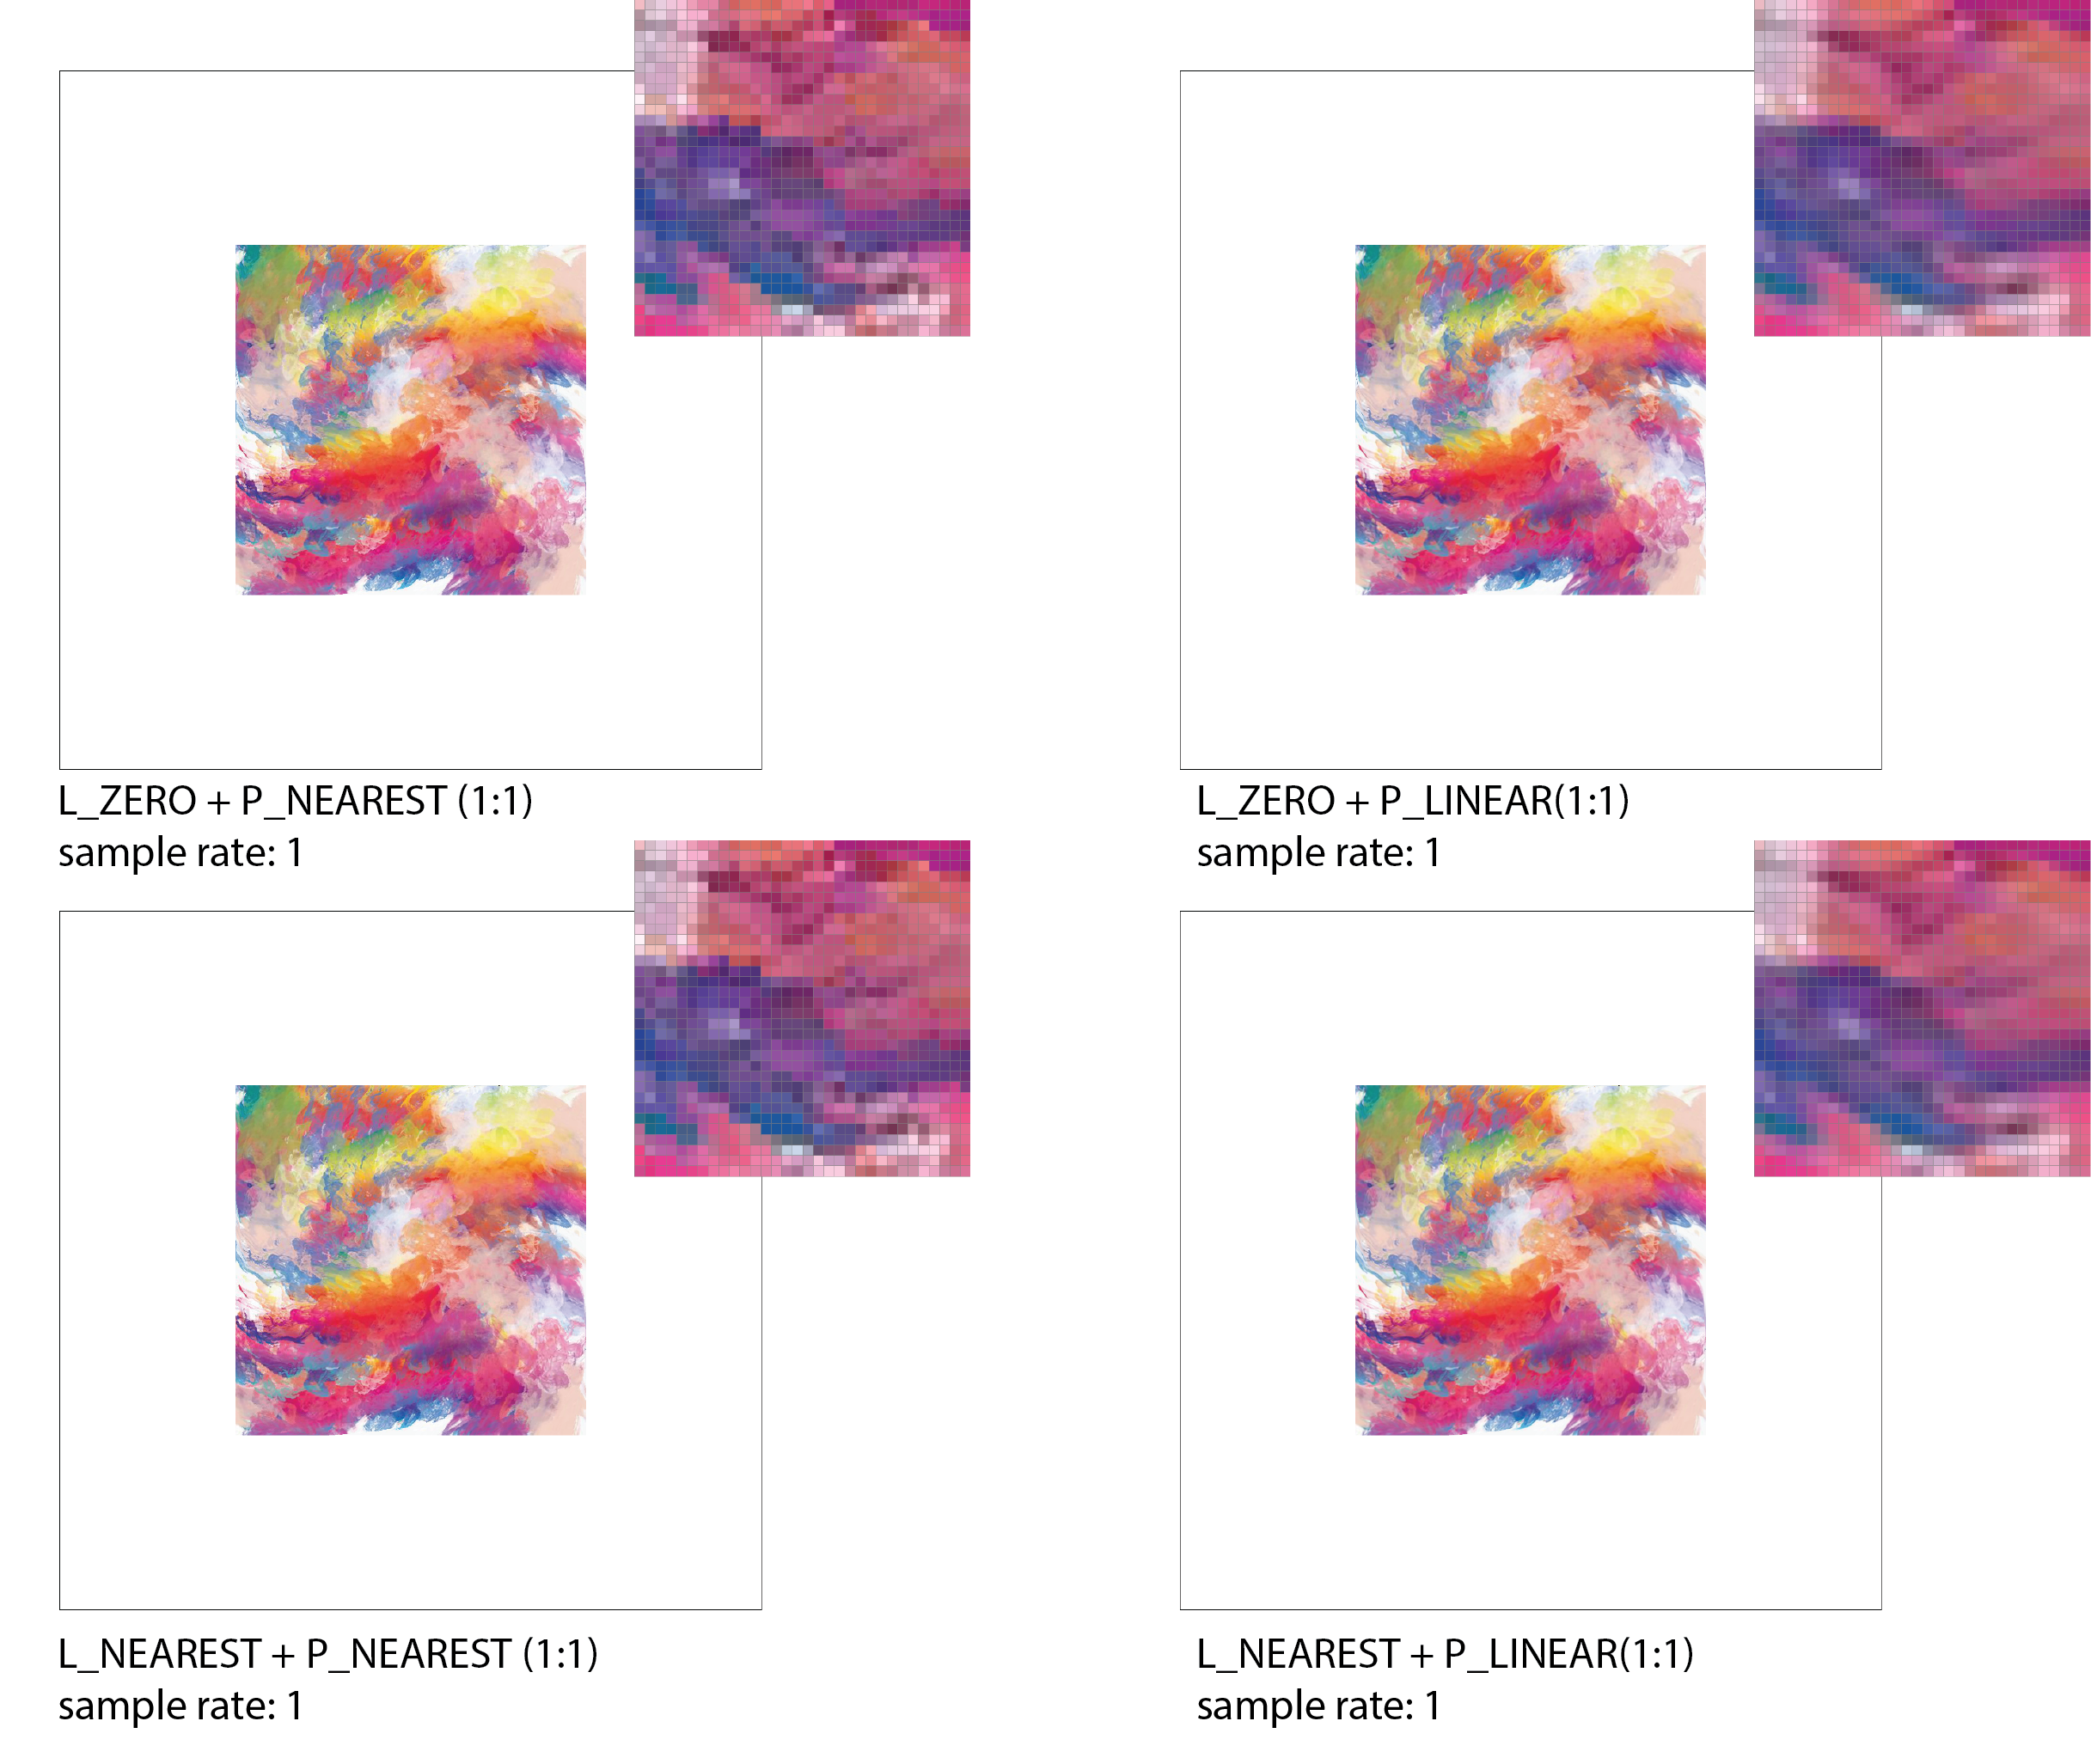
\includegraphics[width=0.99\textwidth]{T6f1-01.png} % Replace with your file name
  \end{figure}
\end{document}


%%% Local Variables:
%%% mode: latex
%%% TeX-master: t
%%% End:
